\documentclass[11pt]{article}
\usepackage[utf8]{inputenc}
\usepackage[T1]{fontenc}
\usepackage{lmodern}
\usepackage[margin=1in]{geometry}
\usepackage{amsmath,amssymb}
\usepackage{booktabs}
\usepackage{graphicx}
\usepackage[numbers,sort&compress]{natbib}
\usepackage[hidelinks]{hyperref}
\usepackage{microtype}
\hypersetup{pdftitle={Adaptive-Rank Decentralized LoRA under Quantity Skew: An SST-2 Benchmark},pdfauthor={AH-LoRA Project Team},pdfsubject={A standalone five-seed comparison of adaptive ranks and sample-size weighting with independently reconstructed Dec-LoRA}}
\newcommand{\R}{\mathbb{R}}
\newcommand{\norm}[1]{\left\lVert#1\right\rVert}
\newcommand{\clip}{\operatorname{clip}}
\newcommand{\median}{\operatorname{median}}
\title{Adaptive-Rank Decentralized LoRA under Quantity Skew:\\An SST-2 Benchmark}
\author{AH-LoRA Project Team}
\date{September 2026}
\begin{document}
\maketitle

\begin{abstract}
Unequal dataset sizes and adapter-rank limits are practical constraints in decentralized fine-tuning. We test whether capability-bounded rank adaptation and sample-size-weighted aggregation provide a useful accuracy--communication tradeoff against an independent reconstruction of Dec-LoRA. RoBERTa-base is trained on SST-2 using ten ring-connected clients with label-stratified, unequal shards. Seven methods are evaluated at five paired seeds, separating rank adaptation and sample weighting, with a separate equal-size reconstruction anchor. Adaptive rank with sample weighting attains $94.243\pm0.249\%$ best validation accuracy, versus $94.541\pm0.238\%$ for rank-16 Dec-LoRA. The paired difference is $-0.298$ percentage points with an unadjusted 95\% interval of $[-0.755,0.159]$, which does not establish equivalence. Training traffic is 31.81\% lower, but the feasible rank-4 comparator reaches $94.495\pm0.334\%$ and requires less traffic: the proposal sends 8.92\% more. The proposal's final-round deficit to rank 16 is $0.550$ points, and sample weighting has no demonstrated accuracy benefit in the factorial comparison. All 36 full-budget runs complete; separate inference audits reproduce predictions from all 72 best/final checkpoints. The study establishes a functioning protocol and a measured tradeoff relative to rank 16, but neither superiority nor a better feasible accuracy--communication tradeoff. Evaluation uses the official labeled validation set and simulated peer transport; it supplies no hidden-test, independent-device memory, or privacy guarantee.
\end{abstract}

\section{Introduction}
Low-rank adaptation (LoRA) fine-tunes a pretrained model through trainable low-rank updates while freezing its original parameters~\citep{hu2022lora}. Federated optimization lets participants optimize on locally owned examples~\citep{mcmahan2017fedavg}; decentralized protocols exchange updates between peers instead of requiring a dedicated aggregation server. A useful system should accommodate participants with different resource budgets and different amounts of data without an unacceptable accuracy penalty.

These constraints interact. A small adapter can limit representational capacity, while averaging heterogeneous low-rank states repeatedly projects shared information into different subspaces. Dataset-size weights also change the stationary distribution of graph mixing. Separate LoRA-factor averages and averages of their matrix products are different operations, even when ranks agree. Finally, a factor-only communication account can overstate savings if a trainable classifier and model assembly are omitted.

We examine these issues on one shared language task with deliberately unequal, label-stratified client shards. The comparator is Dec-LoRA's published RoBERTa-base/SST-2 ring setting~\citep{ghiasvand2025declora}. Our proposed combination uses a stateful, capability-bounded rank controller, static sample-size weights, reversible neighbor mixing, compact product-space aggregation, and a final model assembled by a participating peer. The objective is competitiveness with a conventional decentralized method; an improvement over pooled-data training is not required or tested.

The experiment includes seven methods at seeds 42--46, with matched partitions, client sample streams, optimizer conventions, and local step budgets. A four-arm factorial separates adaptation and weighting, while uniform-rank references distinguish unconstrained accuracy from feasibility at every client. Serialized training messages, classifier traffic, and delivery costs are recorded alongside best and final validation accuracy. All methods and all seeds are retained, including unfavorable outcomes.

The contribution is an auditable empirical comparison of the combined protocol, rather than a new consensus principle or a convergence theorem. The proposed method trains successfully but does not demonstrate an advantage over the feasible rank-4 baseline. This distinction between completing an experiment and confirming its hypothesis is central to the interpretation.

\section{Related Work and Comparator Scope}
Dec-LoRA performs local fine-tuning followed by separate neighbor averages of the two LoRA factors~\citep{ghiasvand2025declora}. We select the REALM 2025 publication because it directly studies decentralized low-rank fine-tuning and reports a tractable RoBERTa-base/SST-2 ring experiment. No author implementation was verified. Our baseline is therefore an independent reconstruction with disclosed assumptions, not an exact numerical reproduction. We pin the workshop version and do not combine its settings with changed scores in later arXiv versions.

Effective-product consensus followed by low-rank factorization is already central to DeCAF~\citep{saadati2025decaf}. Product-space aggregation is not claimed as a novel mechanism here. Our unrestricted product-space arm is a mechanism control on the Dec-LoRA task, not a reproduction of DeCAF's CLIP or LLaMA experiments. Likewise, weights proportional to dataset size are standard empirical-risk weights~\citep{mcmahan2017fedavg}. Static client quantities produce static sample weights, not a learned or dynamic domain-allocation policy.

RoBERTa supplies the pretrained backbone~\citep{liu2019roberta}, and SST-2 in GLUE supplies the task and accuracy endpoint~\citep{wang2019glue}. The scientific question is whether the specified adaptive rank policy, established weighting rule, and graph-constrained aggregation jointly improve the measured tradeoff over simpler decentralized alternatives under controlled quantity skew.

\section{Methodology}
\subsection{Objective and adapted model}
Let $N=10$ clients own disjoint training shards $\mathcal D_i$ of size $n_i$, with $n=\sum_i n_i$. For mean cross entropy $F_i$, the sample-weighted target is
\begin{equation}
 F_i(\theta)=\frac1{n_i}\sum_{(x,y)\in\mathcal D_i}\ell(f_\theta(x),y),
 \qquad F(\theta)=\sum_i\pi_iF_i(\theta),\quad \pi_i=\frac{n_i}{n}.
 \label{eq:objective}
\end{equation}
Uniform-weight controls instead use $\pi_i=1/N$. This states the intended empirical weighting; finite local Adam steps, neighbor mixing, and rank projection do not exactly reproduce centralized optimization of $F$.

LoRA is applied to query and value projections in all 12 RoBERTa-base blocks. For adapted layer $\ell$ and client $i$, the update and layer map are
\begin{equation}
 X_{i\ell}=\frac{\alpha}{r_i}B_{i\ell}A_{i\ell},\qquad
 h_\ell'=\left(W_{0\ell}+X_{i\ell}\right)h_\ell+b_{0\ell},\qquad\alpha=16.
 \label{eq:model}
\end{equation}
Here $A_{i\ell}\in\R^{r_i\times768}$ and $B_{i\ell}\in\R^{768\times r_i}$. The pretrained backbone and projection bias $b_{0\ell}$ are frozen. The complete RoBERTa classification head is trainable: its dense projection and output-layer weights and biases are collected in $\vartheta_i$. Its tanh and dropout operations have no trainable parameters. Gradients propagate through the adapted transformer layers.

\subsection{Sample-size-weighted neighbor mixing}
Peers form an undirected ring with symmetric proposal $Q_{ii}=Q_{i,i-1}=Q_{i,i+1}=1/3$, using indices modulo $N$. A reversible Metropolis--Hastings correction enforces the chosen positive stationary weights:
\begin{equation}
 P_{ij}=Q_{ij}\min\left(1,\frac{\pi_j}{\pi_i}\right)\quad(i\ne j),\qquad
 P_{ii}=1-\sum_{j\ne i}P_{ij}.
 \label{eq:weighted-mh}
\end{equation}
This matrix is row stochastic and preserves the ring's support. Symmetry of $Q$ gives
\begin{equation}
 \pi_iP_{ij}=Q_{ij}\min(\pi_i,\pi_j)=\pi_jP_{ji},\qquad \pi^\top P=\pi^\top.
 \label{eq:detailed-balance}
\end{equation}
Uniform weights yield $P=Q$; sample weights generally produce a matrix that is neither symmetric nor doubly stochastic. Training counts are exchanged once between neighbors. Their ratios suffice for Equation~\eqref{eq:weighted-mh}, and quantities remain fixed throughout each run. Quality scores used below do not enter the sample weights.

Weighting also changes mixing speed. For $D_\pi=\operatorname{diag}(\pi)$, $S_\pi=D_\pi^{1/2}PD_\pi^{-1/2}$ is symmetric. We log its absolute spectral gap $1-\max_{\lambda\ne1}|\lambda(S_\pi)|$ and the post-merge adapter disagreement
\begin{equation}
 V=\sum_i\pi_i\sum_\ell\left\|X_{i\ell}-\sum_j\pi_jX_{j\ell}\right\|_F^2.
 \label{eq:disagreement}
\end{equation}
Thus the sample-versus-uniform comparison changes both the objective weights and graph mixing, rather than isolating the objective alone.

\subsection{Factor and effective-product aggregation}
After local training, common-rank Dec-LoRA averages factors and the classifier separately:
\begin{equation}
 A_{i\ell}^{+}=\sum_jQ_{ij}A_{j\ell}^{\rm local},\quad
 B_{i\ell}^{+}=\sum_jQ_{ij}B_{j\ell}^{\rm local},\quad
 \vartheta_i^{+}=\sum_jQ_{ij}\vartheta_j^{\rm local}.
 \label{eq:factor}
\end{equation}
Effective-product arms instead mix the scaled updates before truncating to each receiver's rank:
\begin{equation}
 Y_{i\ell}=\sum_jP_{ij}X_{j\ell}^{\rm local},\qquad
 X_{i\ell}^{+}=\mathcal C_{r_i}(Y_{i\ell}),\qquad
 \vartheta_i^{+}=\sum_jP_{ij}\vartheta_j^{\rm local}.
 \label{eq:product}
\end{equation}
If $Y=U\Sigma V^\top$, $\mathcal C_r(Y)=U_{:r}\Sigma_{:r}V_{:r}^\top$ is its best rank-$r$ approximation in Frobenius norm, with discarded energy $\sum_{k>r}\sigma_k(Y)^2$. Factor averaging includes cross-products absent from product averaging:
\begin{equation}
 \left(\sum_jw_jB_j\right)\left(\sum_kw_kA_k\right)
 =\sum_{j,k}w_jw_kB_jA_k.
\end{equation}
Moreover, $(B,A)$ and $(BT,T^{-1}A)$ represent the same product for any invertible $T$ but need not produce the same factor average. Product aggregation removes this dependence from the merge itself, although local optimization and the factor-gradient rank statistic remain coordinate-dependent.

For compact merging, let $w_j$ be the receiver's $P_{ij}$, or the final assembly weight $\pi_j$. Concatenate the weighted factors:
\begin{equation}
 L=[\sqrt{w_j\alpha/r_j}\,B_j]_j,\qquad
 R=[\sqrt{w_j\alpha/r_j}\,A_j^\top]_j,\qquad Y=LR^\top.
\end{equation}
Thin QR gives $L=Q_LR_L$ and $R=Q_RR_R$. If $R_LR_R^\top=U\Sigma V^\top$, then
\begin{align}
 \mathcal C_r(Y)&=(Q_LU_{:r})\Sigma_{:r}(Q_RV_{:r})^\top,\\
 B'&=\frac{(Q_LU_{:r})\Sigma_{:r}^{1/2}}{\sqrt{\alpha/r}},\qquad
 A'=\frac{\Sigma_{:r}^{1/2}(Q_RV_{:r})^\top}{\sqrt{\alpha/r}}.
 \label{eq:compact}
\end{align}
The implementation is algebraically the dense truncated SVD, without materializing a dense $768\times768$ update at every merge. Its core dimensions grow with the sum of contributing ranks, so compactness is not a universal workspace bound. Independent dense-oracle checks cover heterogeneous ranks, weights, scaling, gauge changes, and truncation.

Before compression, Equation~\eqref{eq:detailed-balance} preserves the weighted mean. Compression changes it by exactly
\begin{equation}
 \sum_i\pi_iX_i^+-\sum_i\pi_iX_i^{\rm local}
 =\sum_i\pi_i\bigl[\mathcal C_{r_i}(Y_i)-Y_i\bigr].
\end{equation}
These identities do not establish convergence or accuracy parity when local optimization and heterogeneous projection are interleaved.

\subsection{Capability-bounded adaptive rank}
Client ceilings are $R_i^{\max}\in\{4,8,16\}$, with capability index $c_i\in\{0,1/2,1\}$ respectively. All 24 adapted layers at one client share its current rank. The candidate menu and persistent minimum are
\begin{equation}
 \mathcal R_i=\{r\in\{2,4,6,8,12,16,24,32\}:r\le R_i^{\max}\},\qquad
 m_i=\min\{r\in\mathcal R_i:r\ge R_i^{\max}/2\}.
\end{equation}
Ceilings are adapter-rank constraints, not measured limits on total device memory. Fixed heterogeneous controls train at these ceilings. Adaptive clients start at the ceiling and hold it for two warm-up rounds.

Before each local update sequence, a temporary ceiling-rank adapter is evaluated on one fixed, seeded minibatch of 32 local training examples in evaluation mode. For every $A$ and $B$ gradient matrix $G$, including zero gradients, define
\begin{equation}
 s(G)=\frac{\norm{G}_F^2}{\max\{\norm{G}_2^2,10^{-30}\}},\quad s(0)=0,
 \qquad s_i^t=\median_{G\in\mathcal G_i^t}s(G).
 \label{eq:stable-rank}
\end{equation}
The set $\mathcal G_i^t$ contains all 48 factor gradients, not the classifier gradients. At zero-$B$ initialization, zero $A$ gradients remain in this median. Nonfinite demand is replaced by zero; the clipped demand and moving average are
\begin{equation}
 d_i^t=\clip(s_i^t,0,R_i^{\max}),\qquad
 \bar d_i^1=d_i^1,\quad \bar d_i^t=0.7\bar d_i^{t-1}+0.3d_i^t\quad(t>1).
\end{equation}
With $f_i=\max\{2,0.5c_iR_i^{\max}\}$, the candidate is
\begin{equation}
 \widetilde r_i^t=\operatorname{nearest}_{\mathcal R_i}
 \left(\max\{f_i,\min(\bar d_i^t,R_i^{\max})\}\right).
 \label{eq:rank-target}
\end{equation}
Ties choose the smaller menu value; if quantization falls below $f_i$, the smallest menu value at least $f_i$ is used. For current rank $r_i$, the request direction is
\begin{equation}
 z_i^t=\begin{cases}
 +1,&\widetilde r_i^t>r_i\ \text{and}\ \bar d_i^t\ge1.10r_i,\\
 -1,&\widetilde r_i^t<r_i\ \text{and}\ \bar d_i^t\le0.85r_i,\\
 0,&\text{otherwise}.
 \end{cases}
\end{equation}
Two consecutive nonzero requests in the same direction move one menu step, clipped to $[m_i,R_i^{\max}]$. A zero request clears the streak; a direction change starts a new streak. After a step, the streak is reset. Optional residual-demand modulation in the generic controller is disabled.

After local training, the same fixed minibatch supplies quality feedback
\begin{equation}
 q_i^t=(1+\ell_i^t)^{-1},\qquad
 \bar q_i^1=q_i^1,\quad \bar q_i^t=0.8\bar q_i^{t-1}+0.2q_i^t.
\end{equation}
If $q_i^t<0.95\bar q_i^{t-1}$, the next decision restores the ceiling immediately before considering reductions and clears the alarm. Warm-up likewise forces the ceiling. This quality guard affects ranks only; the sample weights remain $n_i/n$. Validation examples never enter the probe, quality guard, or rank policy.

For an increase $r\to r'$, existing $A$ rows and $B$ columns are each multiplied by $\sqrt{r'/r}$. New $A$ rows receive seeded Gaussian values, while new $B$ columns are zero. The current effective update in Equation~\eqref{eq:model} is preserved, with nonzero directions available for subsequent learning. A decrease uses the compact truncated SVD. Ceiling-rank demand probes and forward quality checks add work beyond local training. A lower persistent rank therefore does not establish lower total computation or peak memory. Stable rank of factor gradients is a heuristic demand signal, not an invariant estimate of the uniquely necessary global rank.

\subsection{Final peer assembly and resource accounting}
The first capacity-16 peer is selected before training as the deployment root. After each round, serialized factor and classifier records are gathered along a breadth-first spanning tree of the ring. Relay peers route the records without intermediate adapter truncation. For product-space arms, the root forms
\begin{equation}
 \widehat X_\ell=\mathcal C_{16}\left(\sum_i\pi_iX_{i\ell}\right),\qquad
 \widehat\vartheta=\sum_i\pi_i\vartheta_i.
 \label{eq:assembly}
\end{equation}
For Dec-LoRA, it instead forms $\widehat A_\ell=N^{-1}\sum_iA_{i\ell}$ and $\widehat B_\ell=N^{-1}\sum_iB_{i\ell}$ with a uniform classifier average. Dec-LoRA4 deploys at rank 4. The assembled model is evaluated at the root; it is neither broadcast to weaker peers nor fed back into training. Final assembly is thus part of the peer protocol, rather than an uncharged evaluator-only average.

Every nonlocal training contribution is actually serialized, hashed, decoded, and routed on a declared edge inside the simulator. Let $H=592{,}130$ denote the full classifier parameter count and $M_{ji}^t$ the measured metadata length for directed edge $j\to i$. With fp32 tensors, the training and delivery costs are
\begin{align}
 B_{\rm train}&=\sum_{t=1}^{20}\sum_{j\to i}\left[4\{24\cdot1536r_j^t+H\}+M_{ji}^t\right],\\
 B_{\rm delivery}&=320+B_{\rm train}+B_{\rm final\ gather}.
 \label{eq:bytes}
\end{align}
The 320-byte setup allowance models twenty fixed-width neighbor-count records and is not measured by the model-message serializer. Earlier evaluation gathers are reported separately and excluded from delivery, which includes one final gather. Provisioning the base model, initial state and graph, network framing, and subsequent dissemination are excluded. Reported GB are decimal $10^9$ bytes.

Rank--example products $\sum_{t,i}r_i^t e_i^t$, where $e_i^t$ is the number of local training examples processed, describe adapter work only. They omit the shared backbone, classifier, ceiling probes, quality checks, and merging. Logical inbox storage and structural QR/SVD workspace estimates are also distinct from measured whole-process CUDA peaks. A single process contains the backbone and multiple simulated peers; its peaks cannot establish independent-client device-memory savings.

\section{Experimental Design}
\subsection{Data, reconstruction assumptions, and optimization}
The pinned model is \texttt{FacebookAI/roberta-base}, revision
\begin{quote}\small\texttt{e2da8e2f811d1448a5b465c236feacd80ffbac7b}.\end{quote}
The pinned dataset is \texttt{nyu-mll/glue}, revision
\begin{quote}\small\texttt{bcdcba79d07bc864c1c254ccfcedcce55bcc9a8c}.\end{quote}
All 67,349 canonical SST-2 training examples are allocated to clients; evaluation uses the official 872 labeled validation examples. The official unlabeled test is not used. The published Dec-LoRA table instead lists 66,675 training and 674 development examples. The source of this discrepancy is unresolved, preventing a direct numerical replication or a claim to beat its printed 93.81\% ring result.

The reconstruction retains ten clients, a ring, rank 16, learning rate $10^{-3}$, batch size 32, and 20 rounds. A separate equal-size anchor interprets the publication's ambiguous $K=1$ as one local epoch per round. Other implementation assumptions are query/value adapters in all 12 blocks, $\alpha=16$, common Gaussian $A$ initialization with standard deviation 0.02 and zero $B$, the complete trainable classification head, maximum token length 128 with dynamic padding, pretrained-model dropout, zero adapter dropout, and fp32 deterministic Torch operations. Rank-16 adapters contain 589,824 parameters; classifier parameters are additional. The publication's rounded 0.60M count does not establish its exact adapter specification.

AdamW uses zero weight decay, constant learning rate, and gradient clipping at norm one. Its moments are reset for every peer in every round in every arm. Resetting avoids stale moments in changed SVD coordinates, but is a disclosed reconstruction choice, not an attributed author setting. The same operating point is used throughout; no comparator-specific tuning is performed. This provides a controlled finite experiment rather than a comparison of each method's optimized performance.

\subsection{Quantity partition and matched budget}
The size-ratio vector is $(1,1,1,1,2,2,2,4,4,4)$. For ratios $v_i$, largest-remainder allocation starts at $n_i=\lfloor nv_i/\sum_jv_j\rfloor$ and assigns the remaining examples to the largest fractional remainders. Bipartite integer rounding sets each client/class count to the floor or ceiling of $n_iN_c/n$, while preserving client totals $n_i$ and global class totals $N_c$. Full source-row memberships verify that the shards are disjoint and exhaustive. Quantity is the designed statistical heterogeneity; topics and label distributions are not deliberately separated.

At seed $s$, partition randomization uses $s+10000$, quantity assignment to ring positions uses $s+20000$, and an independent permutation of ceilings $(4,4,4,4,8,8,8,16,16,16)$ uses $s+30000$. Matched methods reuse all these assignments. Independent shuffling avoids deliberately aligning large datasets with large adapter capacities, without assuming zero realized correlation in every finite assignment.

Every quantity arm performs 211 full local updates of 32 examples per peer per round. Local streams independently reshuffle and continue across epoch boundaries, so smaller shards are revisited more often. Each run therefore performs 42,200 aggregate optimizer steps and 1,350,400 training-example exposures. The equal-size full-epoch anchor performs 1,346,980 exposures. Equal local steps avoid confounding sample weights with longer local trajectories at larger clients. Paired methods share each peer's sample order; rank-dependent computation and additional adaptive probes mean total work is not identical.

\subsection{Compared methods and finite campaign}
Table~\ref{tab:arms} defines the seven methods. The last four form a rank-policy by weighting factorial, holding product-space aggregation fixed. Dec-LoRA16 and Product16/sample exceed weaker clients' declared rank caps; Dec-LoRA4 is feasible at every client. Product16/sample changes both aggregation and weights relative to Dec-LoRA16, so that contrast cannot isolate the effect of factor versus product averaging.
\begin{table}[t]
\centering\small
\caption{Seven matched quantity-skew methods. Sample weights are $n_i/n$; uniform weights are $1/10$. A dagger marks references exceeding some client rank caps.}
\label{tab:arms}
\begin{tabular}{llll}
\toprule
Method & Local rank & Aggregation & Weights\\
\midrule
Dec-LoRA16$^\dagger$ & 16 & factor average & uniform\\
Dec-LoRA4 & 4 & factor average & uniform\\
Product16/sample$^\dagger$ & 16 & product + SVD & sample\\
Fixed/uniform & capability ceilings & product + SVD & uniform\\
Fixed/sample & capability ceilings & product + SVD & sample\\
Adaptive/uniform & controller within caps & product + SVD & uniform\\
Adaptive/sample & controller within caps & product + SVD & sample\\
\bottomrule
\end{tabular}
\end{table}

The prospective protocol was archived before full-budget results. After remote numerical and transport tests and seven bounded smoke runs, seed 42 covers all seven quantity arms and the equal-size anchor. All seven quantity arms are retained at seeds 43--46 regardless of early scores. The completed campaign has 35 matched quantity runs and one separate anchor. No post-hoc accuracy gate or selected seed subset determines replication. Source snapshots and hashes identify the immutable training implementation; smoke runs do not enter scientific aggregates.

\subsection{Endpoints and paired analysis}
If $a_{m,s,t}$ is method $m$'s assembled-model percentage accuracy on the 872 validation examples after round $t$, the primary score follows the publication's best-validation endpoint:
\begin{equation}
 b_{m,s}=\max_{1\le t\le20}a_{m,s,t},\qquad
 d_s=b_{{\rm adaptive/sample},s}-b_{{\rm Dec\text{-}LoRA16},s}.
 \label{eq:endpoint}
\end{equation}
The first occurrence resolves ties. Round-20 accuracy is a required secondary endpoint, and Dec-LoRA4 is the feasible comparator. Each method selects its own best round. For $S=5$ paired seeds, the mean difference, sample SD, and descriptive interval are
\begin{equation}
 \bar d=\frac1S\sum_sd_s,\qquad
 s_d=\sqrt{\frac1{S-1}\sum_s(d_s-\bar d)^2},\qquad
 \bar d\pm t_{0.975,S-1}\frac{s_d}{\sqrt S}.
 \label{eq:interval}
\end{equation}
These unadjusted intervals describe seed variation on one fixed validation set, not sampling uncertainty on a new test population. No prespecified noninferiority margin is available, and none is introduced after results. A nonsignificant difference does not establish parity. Repeated validation selection prevents interpreting the primary endpoint as hidden-test generalization.

For the factorial, let $y_{a,w,s}$ denote best accuracy with adaptive indicator $a\in\{0,1\}$ and sample-weight indicator $w\in\{0,1\}$. Within-seed simple effects are
\begin{equation}
 A_{w,s}=y_{1,w,s}-y_{0,w,s},\qquad
 W_{a,s}=y_{a,1,s}-y_{a,0,s}.
\end{equation}
The adaptation main effect, weighting main effect, and interaction are
\begin{align}
 A_s&=\tfrac12(A_{0,s}+A_{1,s}),& W_s&=\tfrac12(W_{0,s}+W_{1,s}),\\
 I_s&=A_{1,s}-A_{0,s}=W_{1,s}-W_{0,s}.
 \label{eq:factorial}
\end{align}
Equation~\eqref{eq:interval} is applied to each paired contrast; final-accuracy analogues are also archived. These secondary exploratory intervals are not adjusted for multiple comparisons. The one-seed equal-size anchor is excluded from five-seed aggregates and cannot estimate the causal effect of quantity skew by itself.

\section{Results}
\subsection{Accuracy against decentralized comparators}
All 36 full-budget runs completed. A separate fresh-process evaluator reproduced the exact raw prediction vectors of all 72 saved best/final checkpoints and verified their source, data, and checkpoint hashes. Table~\ref{tab:results} and Figure~\ref{fig:accuracy} report every matched method; neither the smoke runs nor the equal-size anchor enters the reported uncertainty.
\begin{table}[t]
\centering\small
\caption{SST-2 quantity-skew results at seeds 42--46. Accuracy is percent, mean $\pm$ sample SD. Best over 20 rounds is primary; round 20 is secondary. Mean traffic is decimal GB. Training includes classifier and metadata; delivery adds modeled setup and one final gather, excluding provisioning. A dagger marks references exceeding some client rank caps.}
\label{tab:results}
\setlength{\tabcolsep}{4pt}
\begin{tabular}{lcccc}
\toprule
Method & Best validation & Final validation & Train GB & Delivery GB\\
\midrule
Dec-LoRA16$^\dagger$ & $94.541\pm0.238$ & $94.450\pm0.320$ & 1.893 & 2.011\\
Dec-LoRA4 & $94.495\pm0.334$ & $94.266\pm0.372$ & 1.185 & 1.259\\
Product16/sample$^\dagger$ & $94.725\pm0.181$ & $94.427\pm0.224$ & 1.893 & 2.011\\
Fixed/uniform & $94.518\pm0.262$ & $94.197\pm0.320$ & 1.468 & 1.556\\
Fixed/sample & $94.404\pm0.126$ & $94.220\pm0.238$ & 1.468 & 1.556\\
Adaptive/uniform & $94.174\pm0.221$ & $93.807\pm0.513$ & 1.296 & 1.373\\
Adaptive/sample & $94.243\pm0.249$ & $93.899\pm0.188$ & 1.291 & 1.368\\
\bottomrule
\end{tabular}
\end{table}

Adaptive/sample's primary paired difference from Dec-LoRA16 is $-0.298\pm0.368$ percentage points, with unadjusted 95\% interval $[-0.755,0.159]$. The interval includes zero, but establishes neither superiority nor equivalence. Its final-round difference is $-0.550\pm0.297$ points, with interval $[-0.919,-0.182]$. Reporting only the selected best score would obscure this less favorable final endpoint.

The feasible Dec-LoRA4 comparator also has higher mean best accuracy. Adaptive minus rank-4 is $-0.252\pm0.348$ points, with interval $[-0.684,0.180]$. Product16/sample attains the highest mean best score, $94.725\pm0.181\%$; adaptive/sample trails it by $0.482$ points, with interval $[-0.877,-0.087]$. Product16/sample's final mean is close in magnitude to Dec-LoRA16's, illustrating the influence of best-round selection. This unrestricted product arm exceeds weaker peers' caps and changes both aggregation and weighting, so it establishes neither a feasible solution nor a single-component explanation.

\begin{figure}[t]\centering
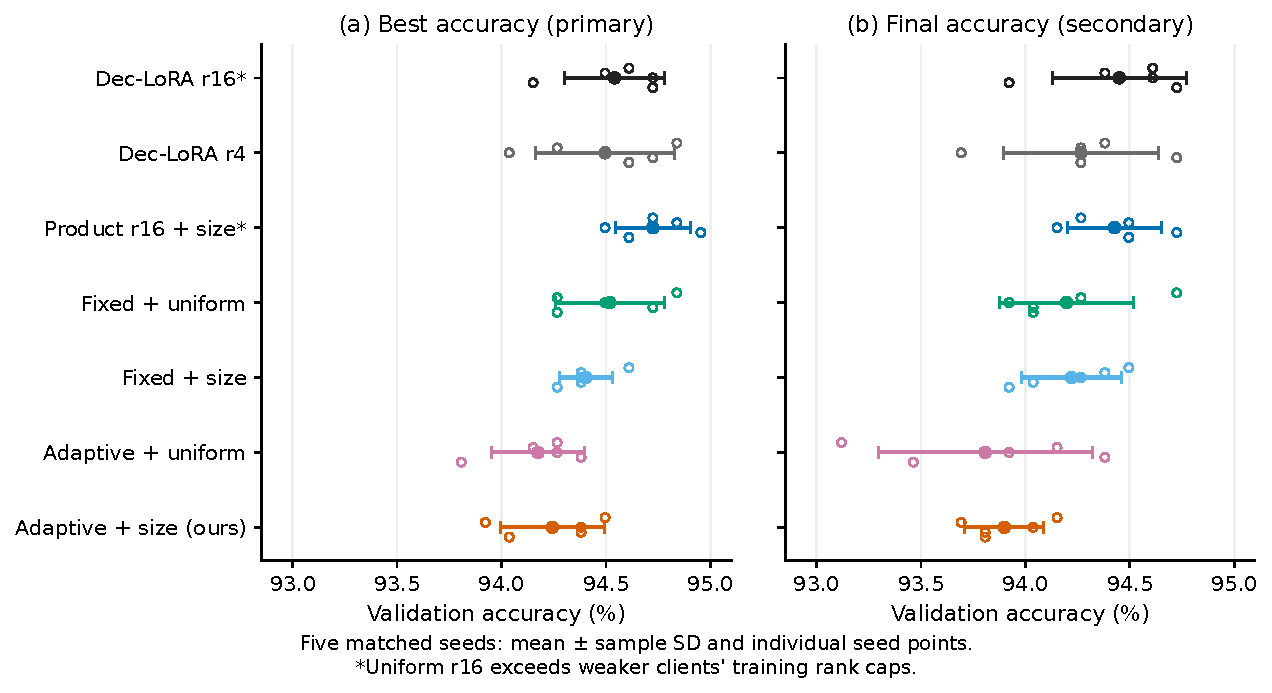
\includegraphics[width=\linewidth]{figures/quantity-skew-accuracy.pdf}
\caption{All seven full-budget methods on official SST-2 validation data. Individual seeds, means, and sample SD distinguish best-round and final-round performance. Rank-16 references exceed weaker peers' caps; the equal-size anchor and smoke runs are excluded.}
\label{fig:accuracy}\end{figure}

\subsection{Rank and sample-weight effects}
Adaptation changes best accuracy by $-0.344$ points at uniform weights (interval $[-0.569,-0.119]$) and by $-0.161$ points at sample weights (interval $[-0.399,0.078]$). Sample weighting changes fixed-rank accuracy by $-0.115$ points (interval $[-0.340,0.110]$) and adaptive-rank accuracy by $+0.069$ points (interval $[-0.169,0.307]$).

The adaptation main effect is $-0.252$ points, with interval $[-0.382,-0.123]$. The weighting main effect is $-0.023$ points, with interval $[-0.152,0.106]$. Their interaction is $+0.183$ points, with interval $[-0.201,0.568]$. These descriptive contrasts (Figure~\ref{fig:effects}) show no demonstrated weighting benefit and a less favorable accuracy pattern for the tested adaptive policy. They do not prove that weighting is universally neutral: quantities, capacities, and ring positions vary jointly across only five seeds, and weighting changes mixing as well as the objective.

\begin{figure}[t]\centering
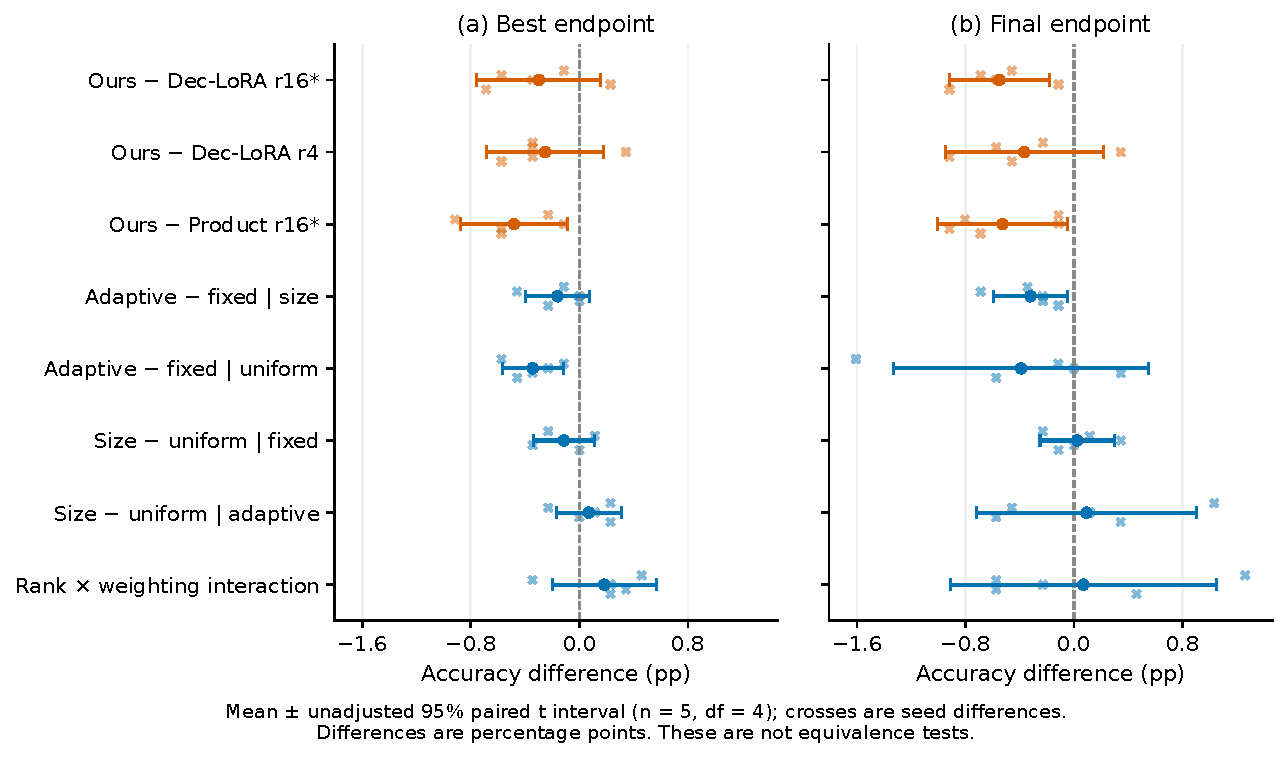
\includegraphics[width=\linewidth]{figures/quantity-skew-paired-effects.pdf}
\caption{Paired comparator and factorial effects in percentage points. Each method uses its own selected best round for primary contrasts. Intervals are unadjusted 95\% Student-$t$ intervals over five seeds, not equivalence tests or hidden-test population intervals.}
\label{fig:effects}\end{figure}

Adaptive/sample's persistent mean training rank is $5.792\pm0.094$, compared with mean ceiling rank 8.8 for fixed heterogeneous training. Its final mean client ranks are 5.6, 5.0, 5.2, 5.4, and 5.4 for seeds 42--46. Figure~\ref{fig:trajectories} shows validation and rank trajectories over the fixed budget. Each adaptive run additionally processes 12,800 probe-example accesses: 6,400 for backward ceiling-rank demand probes and 6,400 for forward quality checks. The common backbone, trainable classifier, and assembly workspace remain. These costs prevent interpreting the persistent-rank reduction as an equal reduction in total FLOPs or independent-device memory.

\begin{figure}[t]\centering
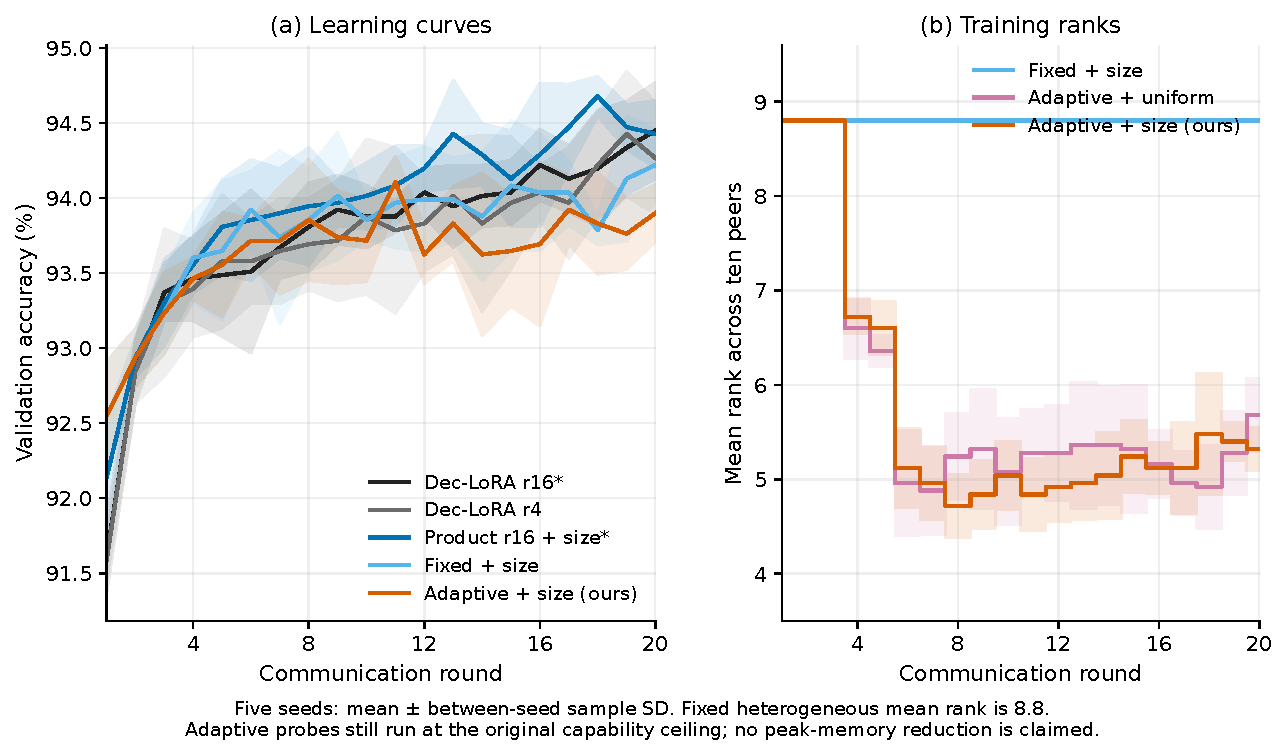
\includegraphics[width=\linewidth]{figures/quantity-skew-trajectories.pdf}
\caption{Validation learning curves and mean client training ranks over 20 rounds. Curves summarize five paired seeds. Evaluation assemblies do not alter training state; displayed training rank excludes ceiling-probe and root-assembly requirements.}
\label{fig:trajectories}\end{figure}

\subsection{Communication tradeoff and reconstruction anchor}
Adaptive/sample sends a mean 1.291 GB during training, 31.81\% less than Dec-LoRA16's 1.893 GB and 12.08\% less than fixed/sample's 1.468 GB. However, it sends 8.92\% more than feasible Dec-LoRA4's 1.185 GB while attaining lower mean accuracy. It therefore offers a measured traffic--accuracy tradeoff relative to rank 16, but does not dominate the simpler rank-4 baseline on either reported accuracy endpoint or training traffic.

The full classifier contributes 0.947 GB to every run's training exchange. Savings computed from adapter factors alone materially overstate total model-message savings. Figure~\ref{fig:tradeoff} retains all methods and identifies the unrestricted rank-16 references. Smaller serialized payloads do not establish a network speedup or device-memory saving.

\begin{figure}[t]\centering
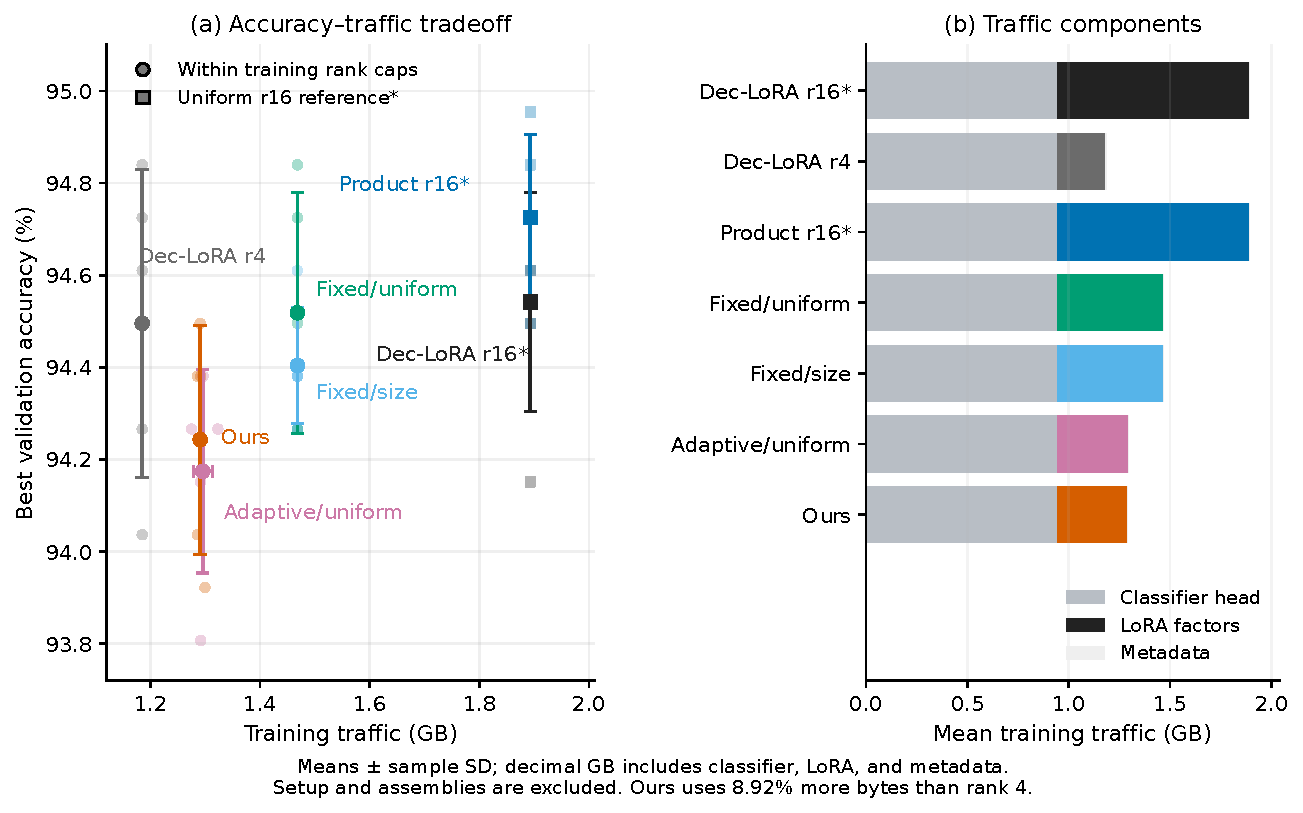
\includegraphics[width=\linewidth]{figures/quantity-skew-tradeoff.pdf}
\caption{Best validation accuracy against serialized training traffic, including adapter factors, the full classifier, and metadata. Provisioning, setup, evaluation gathers, and final delivery are excluded from this axis. Rank 4 is feasible at every declared adapter cap.}
\label{fig:tradeoff}\end{figure}

The equal-size Dec-LoRA16 anchor reaches 94.151\% best and final accuracy at seed 42. It supports the reconstruction's execution but has one seed and slightly different sample exposure from the fixed-step quantity experiment. Its score is not evidence of a win over the publication's 93.81\% result because the canonical split, implementation assumptions, and local-update interpretation differ.

\section{Discussion and Limitations}
The results answer the finite experimental question negatively: the proposed combination does not demonstrate superiority or established parity, and the feasible rank-4 reference has a better observed accuracy--traffic tradeoff. The protocol nevertheless trains useful transformer adapters through graph-constrained exchange. Successful execution should not be confused with confirmation that its extra complexity improves the tradeoff.

The factorial evidence suggests that reducing ranks with this controller is costly at the chosen operating point, while static sample weighting gives no established compensating gain. A gradient stable-rank heuristic need not preserve the directions that matter for prediction after repeated local updates and projections. Quality feedback, floors, and hysteresis mitigate abrupt changes but do not guarantee preservation. The unrestricted product arm performs well, yet its different weights and resource requirements prevent attributing its behavior to product aggregation alone. These are findings about one controller and protocol, not an impossibility theorem for adaptive decentralized LoRA.

The comparator is an independent reconstruction. Unspecified optimizer, classifier, initialization scale, and target-module details, together with the dataset-count discrepancy, limit comparison with the publication's printed score. Common hyperparameters avoid a selective tuning advantage but do not identify each method's best attainable configuration. The one-seed equal-size anchor does not isolate the causal effect of quantity skew. No pooled RoBERTa arm is included, so this study cannot establish equivalence to training a conventional LoRA on the full dataset.

Statistical scope is limited to five seeds, one model family, one task, one topology, one size-ratio schedule, and one capacity schedule. Best-round selection repeatedly uses the same 872 labeled validation examples. The seed intervals neither correct for that selection nor estimate hidden-test generalization, and exploratory secondary contrasts have no multiplicity adjustment. Without a prespecified margin and suitable design, an interval including zero is not a noninferiority result. Broader claims require additional tasks, ratios, topologies, and independently held-out endpoints.

Execution is a single-process simulation on the designated GPU host. Messages are serialized and restricted to graph edges, but the study does not measure physical network latency, asynchronous operation, failures, or independent-host reliability. Adapter-rank caps do not establish that the complete training state fits a particular device. Ceiling probes, classifier state, optimizer work, shared-backbone activations, and final assembly all remain relevant. Whole-process CUDA peaks and structural workspace estimates cannot substitute for independent-client peak-memory measurements.

Each local optimizer reads its assigned shard, and raw examples are absent from peer messages. However, the simulator process can access the whole dataset, and the root sees all routed adapter and classifier records. No differential privacy, secure aggregation, update-leakage assessment, or medical threat model is implemented. Decentralized routing and useful accuracy do not by themselves establish that hospitals or other participants can train without privacy loss.

\section{Conclusion}
The completed five-seed SST-2 benchmark finds that adaptive-rank, sample-weighted decentralized LoRA reaches $94.243\pm0.249\%$ best validation accuracy, compared with $94.541\pm0.238\%$ for reconstructed rank-16 Dec-LoRA. Its 31.81\% lower training traffic accompanies a small observed best-score deficit and a larger final-round deficit. Feasible rank-4 Dec-LoRA reaches $94.495\pm0.334\%$ while using less traffic than the proposal. The experiment therefore does not support superiority, established parity, or a better feasible accuracy--communication tradeoff for the tested combination. All planned runs and checkpoint checks are complete, including unfavorable results. The released protocol, records, and figure data support a reproducible negative comparison and more targeted future work, without a hidden-test or privacy claim.

\section*{Reproducibility and Evidence}
The prospective protocol, immutable launch sources, full memberships, graph records, per-round predictions, rank decisions, sample-order hashes, communication ledgers, and checkpoint audit bindings are archived under \path{docs/artifacts/quantity-skew/}. The training driver is
\begin{quote}\small
\path{project-3-hierarchical-gossip/experiments/quantity_skew_benchmark.py}.
\end{quote}
All experiments, tests, numerical analyses, and figure generation run on \texttt{gpu003}; the 119 remote tests and seven smoke runs support execution validity and are not additional scientific replications. Model and data revisions are stated above. The campaign source identity is
\begin{quote}\small
\path{daced6fc0052f4aab6069aea78ce1468bd5c039b76dedb71080155b0276b8d61}.
\end{quote}

Separate fresh-process checkpoint evaluators reload canonical data and reproduce all 72 best/final prediction vectors. They use separate metric code but share the model architecture and state-install helper, so this is not an independent reimplementation of the entire transformer. The final source-independent artifact audit binds these evaluations to current checkpoint bytes, hashes 36 additional peer-state archives, and reconstructs all 720 saved round accuracy records from stored predictions and canonical validation labels. It also checks partitions, pairing, source identity, and communication arithmetic. That final artifact audit does not itself rerun inference.

Raw wire buffers were not retained; saved payload hashes and ledger consistency are verified without reconstructing every historical message. Initial model-state hashes were also not recorded. Common initialization is supported by source-pinned same-seed code and model tests rather than a per-run initial-state artifact comparison. Large checkpoint binaries remain remotely archived and hash-addressed in repository records; access credentials are not included.

The manuscript's four local figure sets contain PDF/PNG renderings and exact plotted-data JSON. Their reproduction script is \path{scripts/plot_quantity_paper.py}; input/output hashes and statistics are in \path{docs/artifacts/quantity-skew/final-figures/}. The equal-size anchor, smoke runs, and matched quantity runs remain distinct throughout analysis. This standalone manuscript requires only its local \path{references.bib} and \path{figures/} files to compile.

\bibliographystyle{plainnat}
\bibliography{references}
\end{document}
